\chapter{PENDAHULUAN}
\pagenumbering{arabic}
\vspace{4ex}
\label{chap:chap1_introduction}

\section{Latar Belakang}
\vspace{1ex}

Permainan dengan basis \textit{Role-Playing Game} (RPG) adalah permainan yang mana pemain memerankan sebuah karakter khusus dalam sebuah cerita. Pada permainan tersebut, pemain memiliki tujuan untuk menjalankan misi dan mengikuti alur cerita dari permainan tersebut sampai selesai. Terdapat berbagai macam variasi jenis dari RPG, diantaranya adalah WRPG, JRPG, ARPG, SRPG dan MMORPG \citep{stenstrom2012}. 
\vspace{1ex}

Pada Gambar \ref{fig:rpg_turn_based} adalah representasi dari JRPG, yang mana pemain dapat memainkan satu karakter atau lebih. Karakter tersebut melakukan serangan secara bergantian atau \textit{turn-based} antara pemain atau musuh, biasanya musuh yang dilawan berupa \textit{Non-Player Character} (NPC). Bila ditarik garis besar dari jenis permainan RPG tersebut maka dapat digolongkan menjadi 2 yaitu \textit{turn-based} dan \textit{real-time}. Baru saja dijelaskan mengenai \textit{turn-based} sedang untuk \textit{real-time} adalah pertarungan antara pemain dengan musuh dilakukan secara langsung tanpa bergantian. Tipe RPG yang tergolong \textit{turn-based} adalah TRPG dan sebagian JRPG, sedangkan yang tergolong ke dalam \textit{real-time} adalah WRPG, ARPG, SRPG, MMORPG, dan sebagian JRPG.
\vspace{1ex}

\begin{figure} [!h] \centering
	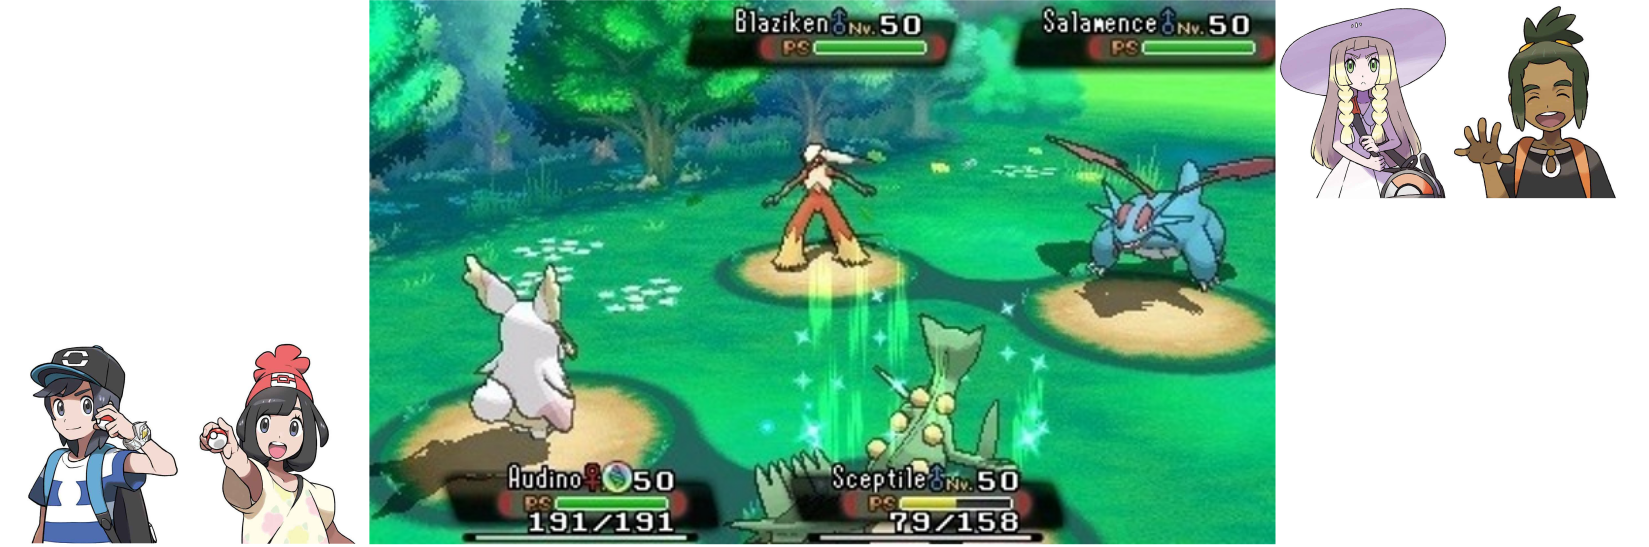
\includegraphics[scale=0.45]{img/turn_based.png}
	\caption{Ilustrasi \textit{turned-based} JRPG}
	\label{fig:rpg_turn_based}
\end{figure}

Dalam sebuah karakter permainan terdapat dua atribut yang berpengaruh yaitu atribut \textit{gameplay} dan atribut estetika. Pada atribut \textit{gameplay} biasanya bersifat non-visual yang menyajikan informasi tentang sebuah karakter dalam sebuah permainan. Sehingga setiap permainan memiliki tipe karakteristik dapat dideskripsikan. Contohnya pada salah satu papan permainan bergenre RPG yang terkenal yaitu \textit{Dungeons and Dragons} \citep{heinsoo2008}, yang memiliki enam atribut \textit{gameplay} seperti \textit{Strength}, \textit{Constitution}, \textit{Dexterity}, \textit{Intelligence}, \textit{Wisdom}, dan \textit{Charisma}. Sedangkan atribut estetika adalah berupa tampilan dari karakter permainan yang meliputi penampilan, warna kulit, pakaian, dan lain sebagainya \citep{camelo2014}. Atribut \textit{gameplay} atau \textit{stats} adalah istilah yang merujuk pada statistik dari fitur yang sesuai dengan karakter seperti ketepatan dalam menggunakan senjata atau keterampilan \textit{magic}. Atribut \textit{gameplay} tersebut berpengaruh pada efisiensi dan kekuatan karakter \citep{wenz2013}. 
\vspace{1ex}

Terdapat juga penjelasan yang menjelaskan tentang atribut \textit{gameplay} atau \textit{stats} dalam permainan adalah angka yang menjelaskan aspek entitas dalam dunia permainan. Entitas pada permainan bisa jadi berupa monster, karakter, senjata, atau mantra. Dalam RPG, biasanya atribut \textit{gameplay} karakter pemain dapat ditingkatkan untuk menguntungkan pemain. Atribut \textit{gameplay} juga digunakan untuk mensimulasikan pertempuran. Jika pemain menyerang karakter musuh, komputer membutuhkan cara untuk memutuskan apakah pemain memukulnya dan jika pemain melakukannya, seberapa banyak kerusakan yang ditimbulkan, dan terakhir perlu memeriksa apakah pukulan itu dapat membunuh musuh atau tidak. Dalam pembuatan keputusan ini, komputer menjalankan kode simulasi dengan menggunakan atribut \textit{gameplay} \citep{danschuller2020}.
\vspace{1ex}

Pada permainan dengan genre RPG yang terdiri dari banyak karakter baik itu karakter pemain dan musuh. Di mana atribut \textit{gameplay} tersebutlah yang akan menentukan jalannya pertarungan antara pemain dan musuh. Kemudian atribut \textit{gameplay} juga menunjukan tingkat kesulitan dari musuh, kelemahan dari musuh, daya tahan musuh terhadap serangan dan lain-lain. Hal ini juga merupakan bagian utama dari desain permainan, yang mana nominal pada atribut \textit{gameplay}, jumlah pemain dan musuh dapat menentukan beberapa faktor penting lain seperti durasi permainan dan alur cerita. 
\vspace{1ex}

Maka dari itu jenis permainan RPG dapat digolongkan juga menjadi 2 golongan lagi berdasar jumlah karakter yang dapat dimainkan oleh pemain yaitu \textit{single-character} dan \textit{multi-character}. Hal ini sangat berkaitan erat dengan penelitian ini saat dilakukannya pengujian, dalam pembuatan atribut \textit{gameplay} untuk pemain harus dibedakan. Tipe RPG yang tergolong \textit{multi-character} adalah TRPG dan JRPG, sedangkan yang tergolong dalam \textit{single-character} adalah WRPG, ARPG, SRPG dan MMORPG.
\vspace{1ex}

Banyak penelitian yang mengaplikasikan berbagai bentuk algoritma dan metode untuk mempercepat pembuatan \textit{video games} sepeti halnya pengukuran tingkat kesulitan dengan menggunakan \textit{challenging rate} (CR) pada permainan 2D \textit{Real Time Strategy} (RTS) \citep{Christyowidiasmoro2016}, pembuatan \textit{game engine} yang berorientasi pada \textit{multi-agent systems} \citep{Marin-Lora2020}, pembuatan level secara otomatis pada permainan secara prosedular dengan tingkat kesulitan tertentu \citep{Wu2018}, pemetaan atribut \textit{gameplay} untuk menentukan estetika karakter secara otomatis dengan menggunakan algoritma fuzzy \citep{camelo2014}, pencapaian keseimbangan dalam permainan \textit{Real Time Strategy} (RTS) dengan pembuatan sebuah \textit{framework} yang dinamakan dengan \textit{attribute space} untuk evaluasi yang direpresentasikan dalam pertarungan \textit{single unit} atau satu lawan satu pada permainan RTS \citep{Bangay2014}. Berdasarkan beberapa penelitian tersebutlah maka penelitian ini dibuat, dengan tujuan memudahkan desainer permainan dalam mendesain sebuah permainan dengan genre RPG.
\vspace{1ex}

Penggunaan berbagai metode seperti $k-$NN, Distribusi Normal dan Naive bayes yang kemudian dilanjutkan dengan diperolehnya atribut \textit{gameplay} untuk pemain dan musuh yang siap digunakan. Kemudian dilanjutkan dengan proses klasifikasi dari atribut \textit{gameplay} tersebut apakah sudah sesuai dengan apa yang direncanakan. Pada proses tersebut digunakanlah \textit{Neural Network Multiclass Classification}.
\vspace{1ex}

\section{Rumusan Masalah}
\vspace{1ex}

Pembuatan atribut \textit{gameplay} untuk karakter yang akan dimainkan oleh pemain dan karakter musuh pada permainan dengan genre RPG yang terkadang masih dilakukan secara manual, terlebih lagi jika karakter dari pemain dan musuh pada permainan tersebut sangat banyak maka diperlukannya sebuah program yang mampu menyusun hal tersebut secara otomatis.
\vspace{1ex}

\section{Tujuan}
\vspace{1ex}

Dari permasalahan yang dirumuskan sebelumnya,maka penelitian ini memiliki tujuan sebagai berikut: 

\begin{enumerate}
	\item Mempercepat proses desain permainan dengan menggunakan program yang dapat menghasilkan atribut \textit{gameplay} yang berupa data statistik untuk karakter dari pemain dan musuh.

	\item Diperolehnya atribut \textit{gameplay} untuk karakter pemain dan musuh yang dihasilkan secara otomatis oleh program dan terklasifikasi bedasarkan tipe yang ingin dibuat.
\end{enumerate}

\section{Batasan Masalah}
\vspace{1ex}

Berdasrkan fokus permasalahan pada bagian sebelumnyaa, kemudian diambilah beberapa pembatasa masalah. Berikut adalah batasan-batasan masalah tersebut.

\begin{enumerate}
	\item Atribut \textit{gameplay} yang dihasilkan oleh program hanya dapat dipakai oleh permainan dengan genre RPG.
	
	\item Program yang dibuat untuk menghasilkan atribut \textit{gameplay} dapat dipakai oleh lebih sama dengan satu karakter pemain dan musuh.

	\item Metode yang digunakan dalam proses perhitungan atribut \textit{gameplay} pemain dan musuh diantaranya adalah $k-$NN, Distribusi Normal dan Naive Bayes.
	
	\item Perhitungan tingkat kesesuaian atribut \textit{gameplay} dari karakter pemain dan musuh yang telah dihasilkan, dengan cara klasifikasi menggunakan \textit{Neural Network Multiclass Classification}.
\end{enumerate}

\section{Kontribusi}
\vspace{1ex}

Di harapkan penelitian ini mampu mejadi rujukan dalam proses desain permainan, khususnya saat pembuatan atribut \textit{gameplay} untuk karakter pemain dan musuh. Selain itu menjadikan proses pengembangan permainan dengan genre RPG di masa mendatang menjadi lebih cepat.
